\chapter{Módszerek}
\pagestyle{headings}
\section{Elektródok}
\subsection{Antimon mikroelektród}
\paragraph{Az antimon mikroelektródok készítése.}
Egy antimonnal töltött boroszilikát üvegkapillárist gázégőn felhevítettem izzásig, majd vékony üvegkapillárist készítettem, úgy, hogy az üvegkapilláris zárt végét csipesszel megfogva hirtelen mozdulattal vékony szálat húztam belőle. A kapott kb. 0,1 mm átmérőjű antimonnal telt kapillárist, mikroszkóp alatt vizsgáltam és kiválasztottam a szakadásmentes részeket, amelyekből 4-5 cm-es darabokat használtam fel alapelektródként. Ezeket az alapelektródokat Amepox A és B komponensének 1:1 arányú keverékével (elektromos vezető epoxi) egy elektromos elvezetés szigetelő műanyagától megfosztott rézhuzalhoz rögzítettem, majd szárítószekrénybe (100 \textdegree C) helyeztem a kétkomponensű ragasztó megkötéséig, ami kb. 1 órát vett igénybe.

\begin{figure}[h]
\centering
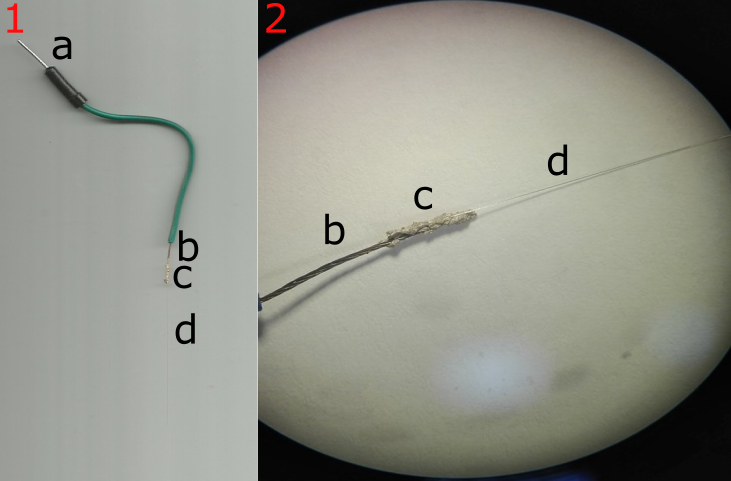
\includegraphics[width=0.5\textwidth]{img/antimon.png}
\caption{Antimon mikroelektród szkennelt és mikroszkópikus képe.}
\label{fig:ionophores}
\end{figure}

\paragraph{Az antimon mikroelektród karakterizálása}
Antimon mikroelektród kalibrálása:\\
A kalibrálást általam készített hét pufferoldat segítségével végeztem, amik körübelül 1 pH egységre álltak egymástól: pH= 3,902; 5,105; 5,442; 6,51; 8,993; 9,464; 10,262. A pontos pH értékeket pH standardokkal kalibráltMethorm pH mérő készülékkel és hozzá tartozó kombinált üvegelektróddal ellenőriztem. A cella összeállítása során a mérőelektród a saját készítésű fém mikroelektród, míg referencia elektródként a pH-méréshez használatos kombinált üvegelektród referencia elektródját használtam.\\
Cella ellenállásának meghatározása feszültségosztó módszerrel:\\
kép...\\
\begin{equation}
R_\text{M} = R_\text{in}
\end{equation}
\begin{equation}
V = \frac{E}{2} = \frac{R_\text{in}}{R_\text{M} + R_\text{in}} * E
\end{equation}
\begin{equation}
R_\text{M} = R_\text{in} (\frac{E}{V} -1)
\end{equation}
A mérést multiméter segítségével végeztem, amit a megfelelő ellenállások használatával és a           multiméter által mért feszültség alapján a fenti egyenletbe helyettesítve meghatározható a cella (fém     mikroelektród és az alkalmazott referencia-elektród) ellenállása. \\
táblázat..\\
Antimon mikroelektród ellenállásának vizsgálata:\\
Kéziműszer segítségével hajtottam végre a mérést, amely során jelen esetben az antimon-elektródot higanyba mártottam. Eleinte „végtelen ellenállást” mértem, majd az elektródból kis darabot letörve valós értéket tudtam mérni. Feltételezhetjük, hogy az antimon-oxidot nem nedvesíti a higany, evvel magyarázható a mérés kezdeti sikertelensége, míg az antimont (frissen letört elektród esetén) nedvesíti a higany.\\
táblázat..\\
Az ellenállás mérés alapján meghatározható az elektród felülete az alábbi egyenlet segítségével: \\
\begin{equation}
R = \rho * \frac{l}{A}
\end{equation}
ahol $R$ az ellenállás, $\rho$ az anyagi minőségre jellemző fajlagos ellenállás, $l$ a hossz és az $A$ a felület. $R = \rho * \frac{l}{A}$-ből $A$-t kifejezve:
\begin{equation}
A = \rho * \frac{l}{R}
\end{equation}
A $\rho$ értéke antimon esetében 417 n\Omega m\\
táblázat..\\
A felületet ismerve meg tudjuk határozni az antimon-elektródok átmérőjét: \\
\begin{equation}
A = \Pi \times r^2
\end{equation}
táblázat..\\
Az antimon átmérőjének meghatározása során feltételeztem, hogy az antimon elektród kör keresztmetszetű, és az elektród folytonos illetve egyenlő vastagságú.

\subsection{Szénszél mikroelektród}
Amepox A és B komponensét 1:1 arányban összekevertem, majd egy gyárilag előállított 33 $\upmu$m átmérőjű szénszálat (Specialty Materials Inc. 1449 Middlesex Street Lowell, Massachusetts 01851) a ragasztó segítségével az elektromos elvezetés szigetelő műanyagától elválasztott rézhuzalhoz rögzítettem. A ragasztó megkötéséig szárítószekrénybe helyeztem az elektródokat (kb. 1 óra). Ezután a szénszálat az elektromos elvezetéssel együtt egy húzott végű boroszilikát üvegkapillárisba helyeztem, úgy, hogy a szénszál kb. 5 mm-t lógjon ki a kapillárisból. A kapilláris végének lezárását egy folyékony kétkomponensű epoxi ragasztóval végeztem (helyi barkácsboltból beszerezve), hogy kis mennyiségű folyékony ragasztót a kapilláris végéhez helyeztem, ami a kapilláris hatás miatt a kapillárisba jut, ezáltal egy zárt képezve a kapilláris végén, ami meggátolja a mérendő oldat kapillárisba jutását.
\begin{figure}[h]
\centering
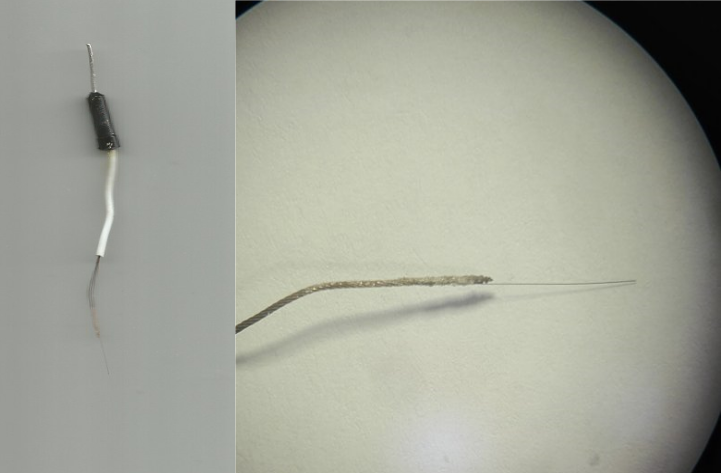
\includegraphics[width=0.5\textwidth]{img/szen33.png}
\caption{33 mikrométeres szén mikroelektród szkennelt és mikroszkópikus képe.}
\label{fig:ionophores}
\end{figure}

\begin{figure}[h]
\centering
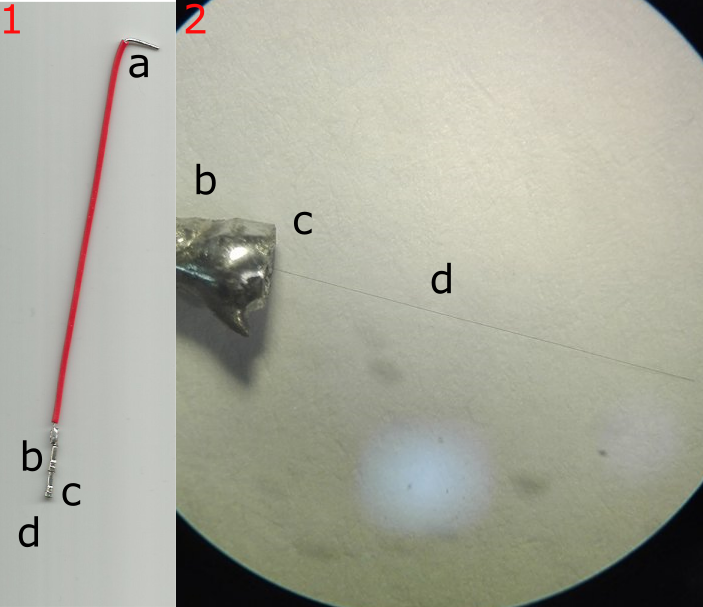
\includegraphics[width=0.5\textwidth]{img/szenmikro.png}
\caption{7 mikrométeres szén mikroelektród szkennelt és mikroszkópikus képe.}
\label{fig:ionophores}
\end{figure}

\paragraph{Válaszidő meghatározása}
Az oszcilláló reakciók tanulmányozása előtt a mérőműszer (potenciosztát) válaszidejét vizsgáltam, annak alkalmasságának bizonyítása végett.
\subsection{Platina mikroelektród}
Gyárilag előállított 25 $\upmu$m átmérőjű platina szálat (Goodfellow Materials) a már jól ismert Amepox A és B komponens 1:1 arányú keverékével ragasztottam egy a szigetelő műanyagától megfosztott elektromos elvezetés réz szálához, amit jól bevált módon kb. 1 órára szárítószekrénybe (100 \textdegree C) helyeztem a kétkomponensű ragasztó megkötéséig.  A megszáradt alapelektródot egy előre kihúzott végű kapillárisba helyeztem, úgy, hogy a platina szál kb. 3-5 mm-re lógjon ki a kihúzott végű kapillárisból. A kapilláris végét folyékony két komponensű ragasztóval zártam le a már fentiekben tárgyalt szénszál mikroelektród készítése alapján. Az elektromos kontaktust ezüst-epoxi (Amepox) biztosította.
\begin{figure}[h]
\centering
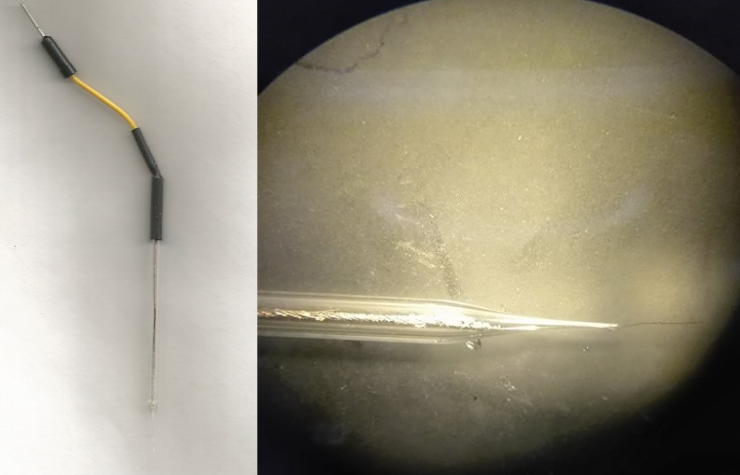
\includegraphics[width=0.5\textwidth]{img/platina.png}
\caption{Platina mikroelektród szkennelt és mikroszkópikus képe.}
\label{fig:ionophores}
\end{figure}
\subsection{Volfrám mikroelektród}
Gázláng felett a kapilláris egyik végét bezártam, majd egy 60 W-os izzóból nyert volfrám szálat helyeztem bele. (1-2 cm) Ezt vákuum alatt hevítem, amit úgy értem el, hogy vízsugár szivattyút egy vékony kis csővel a kapilláris nyitott végéhez kapcsoltam. A hevítés során a volfrám szál kb. felét üvegbe olvasztom, a vákuum hatására a meglágyult üveg és a fémszál buborékmentesen összeolvad. A volfrám másik fele forrasztó ón által fog kapcsolódni az elektromos elvezetéshez, ezt a következőképpen hajtom végre: a kapillárisba cint helyeztem, amit gázláng alatt megolvasztottam, majd leráztam a volfrám üvegbe nem zárt feléhez. Ezután ismét cint helyeztem a kapillárisba majd az elektromos elvezetést, a cint megolvasztva és lerázva kapcsoltam az elektromos elvezetést a volfrám szálhoz.
Az elektród így félkész állapotban van, ugyanis az elején bezárt kapillárisban lévő volfrám szál még nem érintkezik a vizsgálandó oldattal, ezért a fémet borító felesleges üveg lecsiszolásával tudtam a vizsgálandó oldattal érintkezővé tenni. A csiszolást 240-es csiszolópapírral kezdtem, majd P2000-es végül P4000-es nedves csiszoló papírral csiszoltam addig, amíg a véglapon a korong fém megjelent. Ezen műveletek után mérésre alkalmas volfrám elektródot kaptunk.
\begin{figure}[h]
\centering
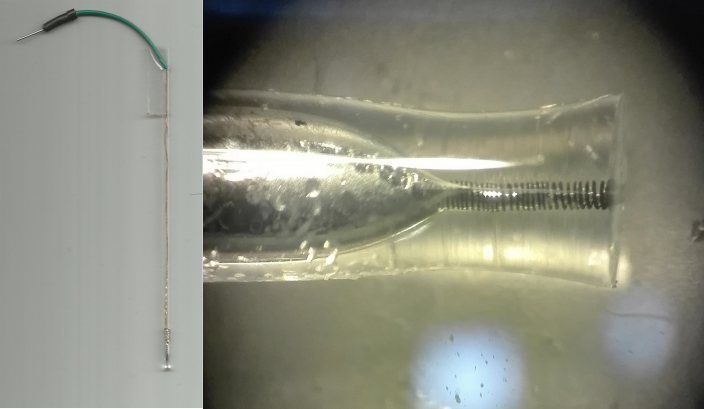
\includegraphics[width=0.5\textwidth]{img/volfram.png}
\caption{Volfrám mikroelektród szkennelt és mikroszkópikus képe.}
\label{fig:ionophores}
\end{figure}

\section{Oszcilláló reakciók tanulmányozása}

Minden oszcilláló reakciót a következő “hardver” és szoftver felhasználásával hajtottam végre. Indikátor elektród(platina,antimon,szén) Ag/AgCl referencia elektród volt az alkalmazott “hardver”.  Az alkalmazott szoftver az EDAQ Chart (Doig Ave, Denistone East NSW 2112, Australia),  méréstartományként 1V-ot alkalmaztam, mintavételezési frekvenciaként 10 Hz-et állítottam be. A mérési adatokat számítógép rögzítette, ami a mérőcellához volt kapcsolva.



\subsection{Makroelektródokkal}
\begin{enumerate}
\item Vizsgálataim során két különböző oszcilláló reakciót tanulmányoztam az általam készített, az előbbiekben említett elektródokkal. 
Először a következő oszcillátor összetételt vizsgáltam.\\
táblázat..\\
Ezek a mennyiségek bemérését meghatározott sorrendben végeztem a következőképpen: Először a kétszer ioncserélt vizet mértem be, majd a malonsavat, kálium-bromátot, kénsavat és végezetül a mangán-szulfátot. A reakció a mangán-szulfát hozzáadása után indult. A reakcióelegyet mágneses keverővel kevertem. Ennek a reakciónak a tanulmázásából messzemenő következtetéseket nem lehet levonni, csak a Field, Noyes és Kőrös által publikált eredmények reprodukálása [2] volt a cél, amint azt már a Oszcilláló kémiai reakciók című fejezetben említettem.
\item A kevertetett reakció esetén spektrofotometriásan meghatároztam a piros illetve a kék szín abszorbciós maximumát.
\end{enumerate}

\subsection{Mikroelektródokkal} 

A Field, Noyes és Kőrös által elért eredmények reprodukálása utána [2] keveretlen közegben vizsgáltam a reakciót.
A továbbiakban vizsgált oszcilláló reakciót kevertetés nélkül, a következő összetételű oldatokkal dolgoztam: [3]

\subsection{Pásztázó elektrokémiai mikroszkóp alkalmazása}



\begin{figure}[h]
\centering
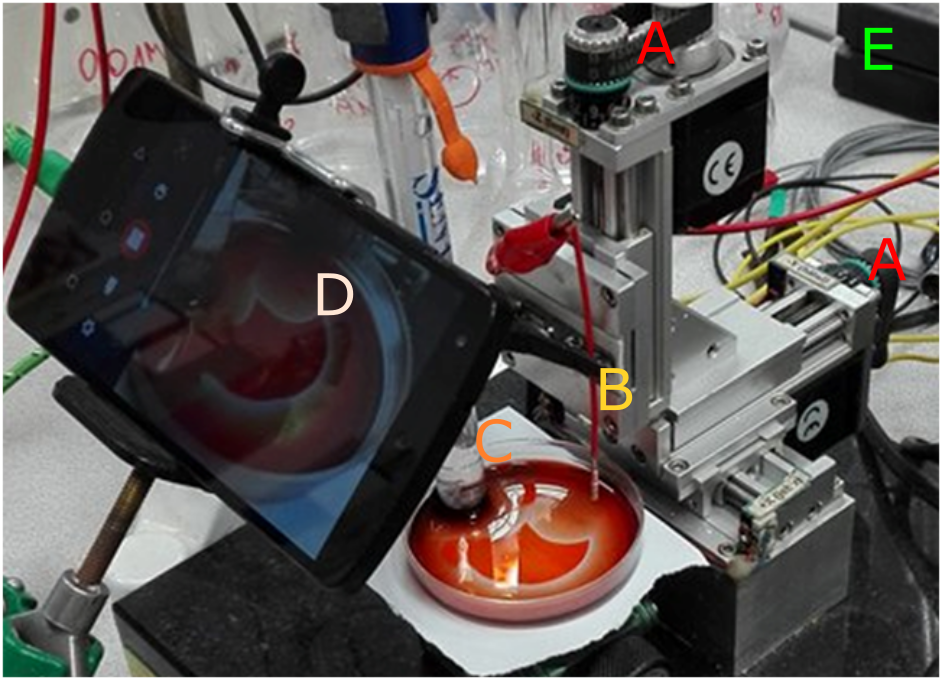
\includegraphics[width=0.8\textwidth]{img/secm.png}
\caption{(A) Léptetőmotorok, (B) indikátor elektród (C) referencia elektród, (D) kamera, (E) nagy bemeneti impedanciájú feszültségmérő.}
\label{fig:secm}
\end{figure}

\begin{table}[]
\centering
\caption{A reakció komponenseinek koncentrációi.}
\label{my-label}
\begin{tabular}{llllll}
Komponens                       & Malonsav & Kálium-bromát & Kénsav & Mangán-szulfát & Ioncserélt víz \\
\hline
Koncentráció (M)                & 1        & 0.2           & 5      & 0.125          & -              \\
Térfogat (cm$^3$) & 12       & 9             & 11     & 6              & 1              \\
\end{tabular}
\end{table}



